%%%%%%%%%%%%%%%% Relojes Bloom.
\begin{frame}[fragile]{Relojes Bloom:}{Filtro Bloom.}
  \justifying
  \textbf{Def.} El \textit{filtro Bloom} es una estructura de datos,
  probabilística, eficiente en espacio diseñada para verificar rápidamente
  si un elemento esta contenido en conjunto.\newline

  \textbf{Algoritmo.}
  \begin{enumerate}
  \item Definir $k$ funciones \textit{HASH} independientes.
  \item Definir un arreglo de \code{bits} con $m$ \code{bits},
    todos inicialmente igual a $0$.
  \item Para agregar un elemento al \textit{filtro bloom}, hacer
    \begin{enumerate}
    \item Pasamos el elemento, digamos $x$, por las $k$ \textit{funciones
      hash}.
    \item Cada hash apunta a un índice en el arreglo de \code{bits}
    \item La posición a la que se apunte cambia de $0$ a $1$.
    \end{enumerate}
  \end{enumerate}

  \begin{figure}
    \centering
    \begin{subfigure}[b]{0.5\textwidth}
      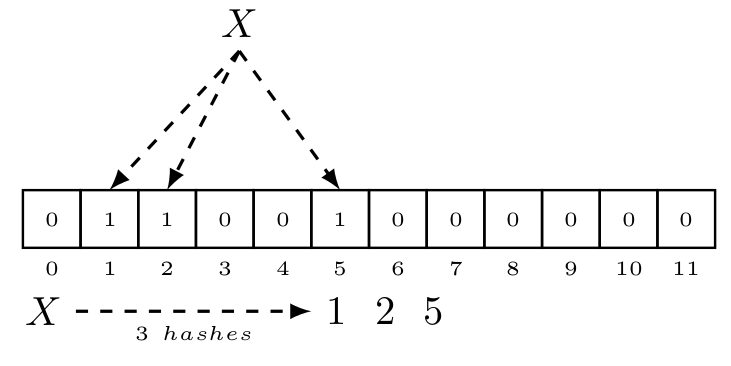
\includegraphics[width=\textwidth]{./Imagenes/Hash01}
      \caption{Inserción al filtro.}
      \label{fig:Ejemplo de Hash(X).}
    \end{subfigure}
  \end{figure}
\end{frame}
